\documentclass{standalone}

\usepackage{pgfplots,tikz,amsmath}
\begin{document}
    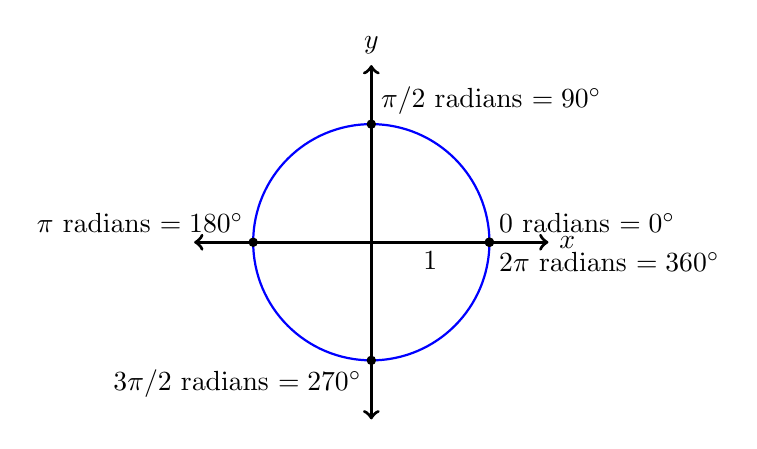
\begin{tikzpicture}[scale=1.5]
        \draw[<->, very thick] (-1.5,0) -- (1.5,0) node[anchor=west]{$x$}; 
        \draw[<->, very thick] (0,-1.5) -- (0,1.5) node[anchor=south]{$y$}; 
        \draw (0.5,0) node[anchor=north]{$1$};
        \draw[thick, color=blue] (0,0) circle(1cm);
        \draw[color=black, fill=black] (1,0) circle(0.035cm) node[anchor=south west]{0 radians
        $=0^\circ$};
        \draw[color=black, fill=black] (1,0) circle(0.035cm) node[anchor=north west]{$2 \pi$ radians
        $=360^\circ$};
        \draw[color=black, fill=black] (0,1) circle(0.035cm) node[anchor=south
        west]{$\pi/2$ radians $=90^\circ$};
        \draw[color=black, fill=black] (-1,0) circle(0.035cm) node[anchor=south
        east]{$\pi$ radians $=180^\circ$};
        \draw[color=black, fill=black] (0,-1) circle(0.035cm) node[anchor=north
        east]{$3\pi/2$ radians $=270^\circ$};
    \end{tikzpicture}
    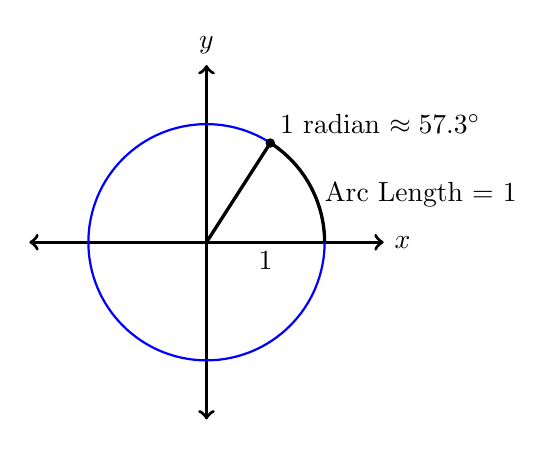
\begin{tikzpicture}[scale=1.5]
        \draw[<->, very thick] (-1.5,0) -- (1.5,0) node[anchor=west]{$x$}; 
        \draw[<->, very thick] (0,-1.5) -- (0,1.5) node[anchor=south]{$y$}; 
        \draw (0.5,0) node[anchor=north]{$1$};
        \draw[thick, color=blue] (0,0) circle(1cm);
        \draw[color=black, very thick] (0,0) -- (0.54,0.84);
        \draw[color=black, fill=black] (0.54,0.84) circle(0.035cm) node[anchor=south
        west]{1 radian $\approx 57.3^\circ$};
        \draw[color=black, very thick] (1,0) arc(0:57.3:1cm);
        \draw[black] (0.92,0.4) node[anchor=west]{Arc Length = 1};
    \end{tikzpicture}
\end{document}
